\begin{table*}[tb]
    \centering
    \fontsize{11}{11}
    \small
	% Model Manufacturer Category PLP-Support Capacitor 
    %\begin{tabular}{p{2.4cm}|p{1.3cm}|p{1.2cm}|l}
    %\begin{tabular}{p{2.4cm}|p{2.4cm}|p{2.4cm}|p{2.4cm}|p{2.4cm}}
    \begin{tabular}{|l|l|l|l|l|l|l|}
    %\begin{tabular}{|p{5cm}|l|l|l|}
        % \hline
        % \multirow{4}{*}{{\rotatebox{90}{\parbox{1.2cm}{\centering \footnotesize{Concurrency}}}}} 
		\hline
		\bf{Workload} & \bf{Reqs.} & \bf{Footprint(D)} & \bf{Footprint(M)} & \bf{Total I/O(D)} &\bf{Total I/O(M)} &\bf{Map-data-ratio(Percentage)} \\ \hline \hline
		fileserver & 4965791 & 1.36GB & 22.27MB & 18.94GB & 346.95MB & 1.79\\ \hline 		
		webserver & 15264309 & 27.81GB & 445.70MB & 58.22GB & 448.15MB & 0.75 \\ \hline 		
		linkbench & 3412657 & 4.00GB & 174.61MB & 13.02GB & 1314.69MB & 9.86 \\ \hline 		
		YCSB-00 & 70682260 & 162.571GB & 332.03MB & 269.63GB & 552.15MB & 0.20 \\ \hline 		
		YCSB-01 & 58037200 & 123.82GB & 252.73MB & 221.39GB & 453.60MB & 0.20 \\ \hline 		
		Systor-16LUN3 & 1200345 & 1.97GB & 89.06MB & 4.58GB & 715.70MB & 15.26 \\ \hline 		
		Systor-16LUN4 & 1000701 & 1.62GB & 61.33MB & 3.82GB & 596.50MB & 15.26 \\ \hline 		
		Systor-18LUN3 & 1464747 & 2.19GB & 83.20MB & 5.59GB & 1044.59MB & 18.26 \\ \hline 		
%        Channel & 8x \\ \hline
%        Way & 4x \\ \hline
%        Die & 4x \\ \hline
%        Plane & 4x \\ \hline
%        Page Size & 4KB \\ \hline
%        SSD Capacity & 512GB \\ \hline
    \end{tabular}
    \caption{\textbf{Workload Characteristics(fifo policy, protected 0.01).}}
    \label{tab:wk_char}
    % \vspace{-10pt}
\end{table*}

\begin{table*}[tb]
    \centering
    \fontsize{11}{11}
    \small

    \begin{tabular}{|l|l|l|l|l|l|l|}
		\hline
		\bf{Workload} & \bf{Reqs.} & \bf{Footprint(D)} & \bf{Footprint(M)} & \bf{Total I/O(D)} &\bf{Total I/O(M)} &\bf{Map-data-ratio(Percentage)} \\ \hline \hline
		random & 5000000 & GB & MB & 19.07GB & 18.88GB & 98.99\\ \hline 		
		fileserver-300s & 1143106 & 1.14GB & 2.41MB & 4.36GB & 9.98MB & 0.22\\ \hline 		
		fileserver-60s & 413613 & 1.04GB & 2.24MB & 1.58GB & 3.65MB & 0.23\\ \hline 		
		linkbench-load & 3456185 & 3.19GB & 6.62MB & 13.18GB & 48.72MB & 0.36\\ \hline 		
		linkbench-run & 3272243 & 3.41GB & 23.11MB & 12.48GB & 1.14GB & 9.11\\ \hline 		
    \end{tabular}
    \caption{\textbf{Workload Charateristics(filesystem aging).}}
    \label{fs_aging} 
\end{table*}	

\begin{figure*}[!bt]
    \centering{}
    \subfloat[Fileserver]{
        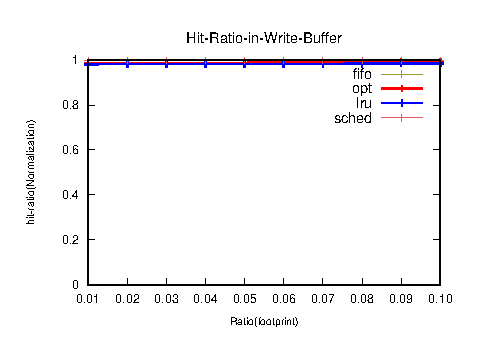
\includegraphics[width=0.24\textwidth]{./hit-eps/fileserver_map.trc.rslt.eps}
	}
    \subfloat[Webserver]{
        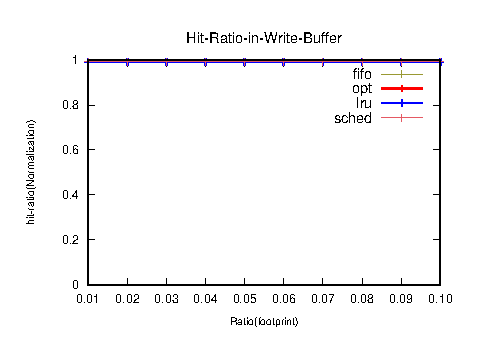
\includegraphics[width=0.24\textwidth]{./hit-eps/webserver_map.trc.rslt.eps}
	} 
    \subfloat[Linkbench]{
        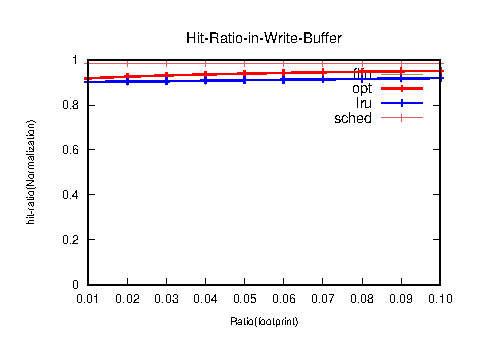
\includegraphics[width=0.24\textwidth]{./hit-eps/linkbench_r_map.trc.rslt.eps}
	}
	\subfloat[YCSB-00]{
        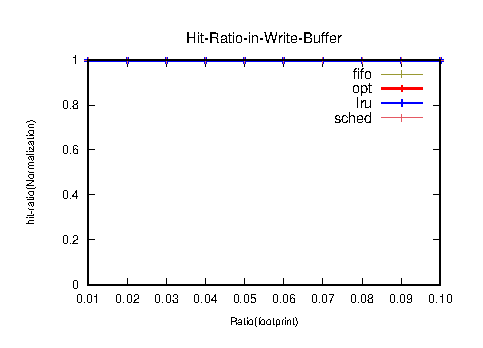
\includegraphics[width=0.24\textwidth]{./hit-eps/ssdtrace-00.blk_w.trc.rslt.eps}
	} \\
	\subfloat[YCSB-01]{
        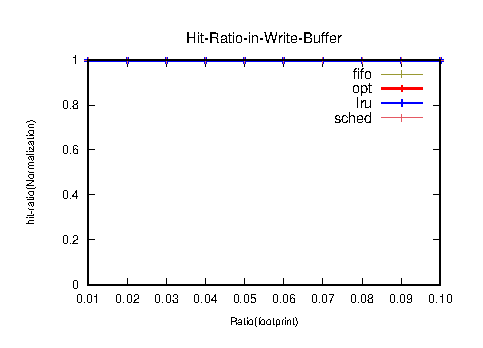
\includegraphics[width=0.24\textwidth]{./hit-eps/ssdtrace-01.blk_w.trc.rslt.eps}
	} 
	\subfloat[Systor-16LUN3]{
        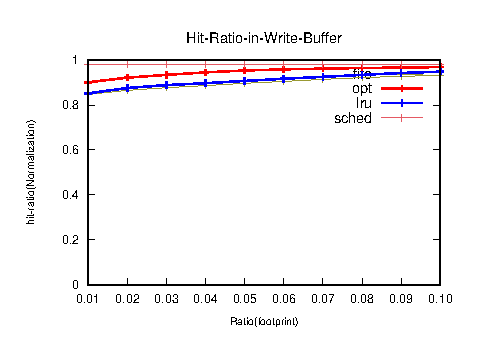
\includegraphics[width=0.24\textwidth]{./hit-eps/2016021616-LUN3.csv_w.trc.rslt.eps}
	} 
	\subfloat[Systor-16LUN4]{
        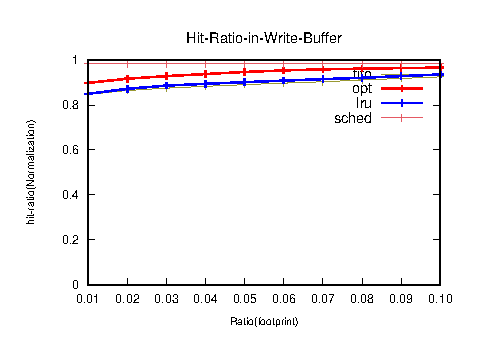
\includegraphics[width=0.24\textwidth]{./hit-eps/2016021616-LUN4.csv_w.trc.rslt.eps}
	} 
	\subfloat[Systor-18LUN3]{
        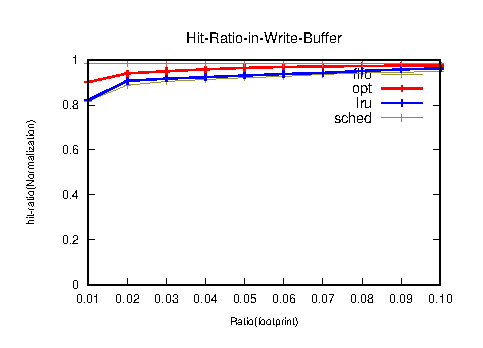
\includegraphics[width=0.24\textwidth]{./hit-eps/2016021618-LUN3.csv_w.trc.rslt.eps}
	} 

	\caption{\textbf{Hit ratio in protected mapping table pages.}
%		\st{The \texttt{fillrandom} inserts items with random keys for each thread,
%    and the \texttt{overwrite} updates existing values in random order.
%    Both represent a put operation.
%    The \texttt{readrandom} retrieves items randomly,
%    and the \texttt{seekrandom} performs random seeks and queries the next ten items.}
	 }\label{fig_hit_ratio}
\end{figure*} 

\begin{figure*}[!bt]
    \centering{}
    \subfloat[Fileserver]{
        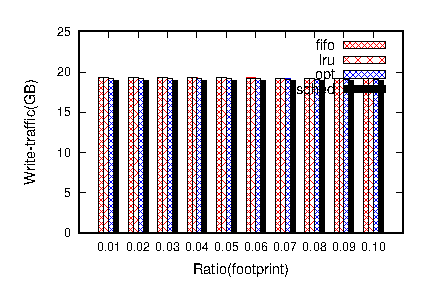
\includegraphics[width=0.24\textwidth]{./total-traffic/fileserver_map.trc.eps}
	}
    \subfloat[Webserver]{
        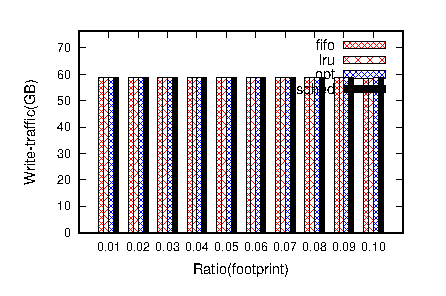
\includegraphics[width=0.24\textwidth]{./total-traffic/webserver_map.trc.eps}
	} 
    \subfloat[Linkbench]{
        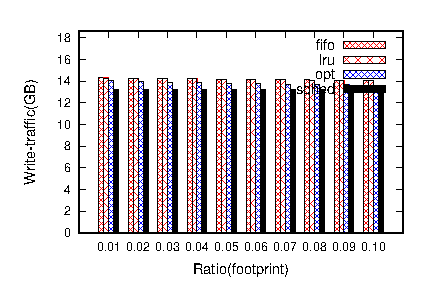
\includegraphics[width=0.24\textwidth]{./total-traffic/linkbench_r_map.trc.eps}
	}
	\subfloat[YCSB-00]{
        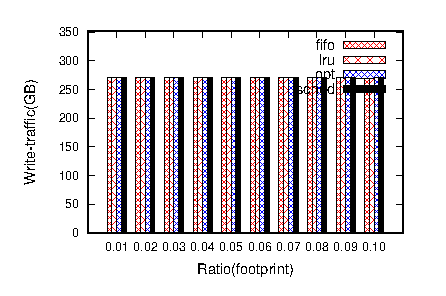
\includegraphics[width=0.24\textwidth]{./total-traffic/ssdtrace-00.blk_w.trc.eps}
	} \\
	\subfloat[YCSB-01]{
        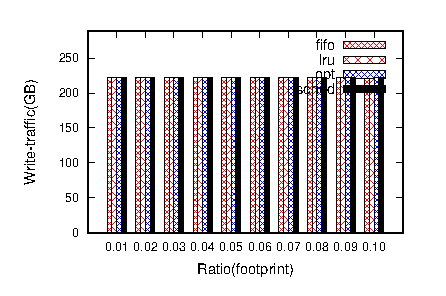
\includegraphics[width=0.24\textwidth]{./total-traffic/ssdtrace-01.blk_w.trc.eps}
	} 
	\subfloat[Systor-16LUN3]{
        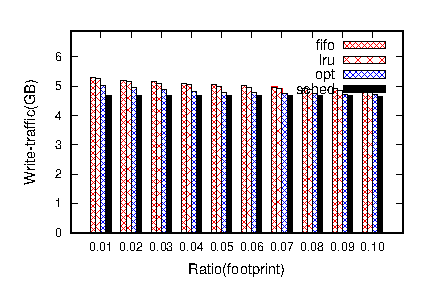
\includegraphics[width=0.24\textwidth]{./total-traffic/2016021616-LUN3.csv_w.trc.eps}
	} 
	\subfloat[Systor-16LUN4]{
        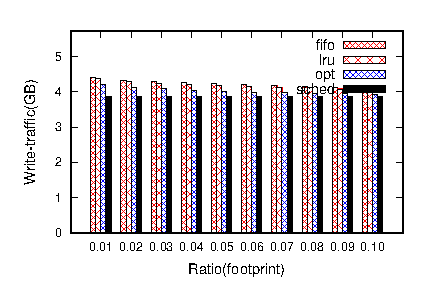
\includegraphics[width=0.24\textwidth]{./total-traffic/2016021616-LUN4.csv_w.trc.eps}
	} 
	\subfloat[Systor-18LUN3]{
        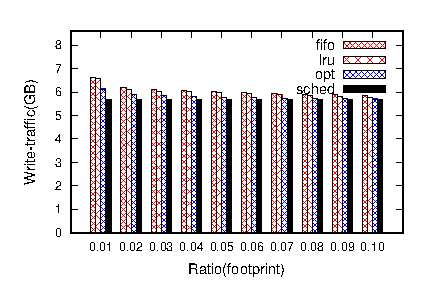
\includegraphics[width=0.24\textwidth]{./total-traffic/2016021618-LUN3.csv_w.trc.eps}
	} 

	\caption{\textbf{Write-back traffic of total data.}
%		\st{The \texttt{fillrandom} inserts items with random keys for each thread,
%    and the \texttt{overwrite} updates existing values in random order.
%    Both represent a put operation.
%    The \texttt{readrandom} retrieves items randomly,
%    and the \texttt{seekrandom} performs random seeks and queries the next ten items.}
	 }\label{fig_total_write_traffic}
\end{figure*} 

\begin{figure*}[!bt]
    \centering{}
    \subfloat[Fileserver]{
        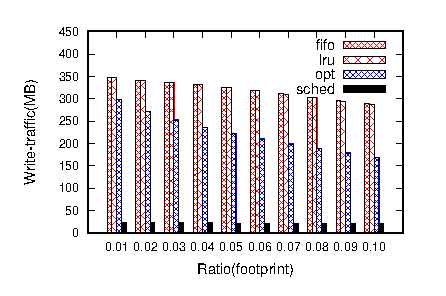
\includegraphics[width=0.24\textwidth]{./map-traffic/fileserver_map.trc.eps}
	}
    \subfloat[Webserver]{
        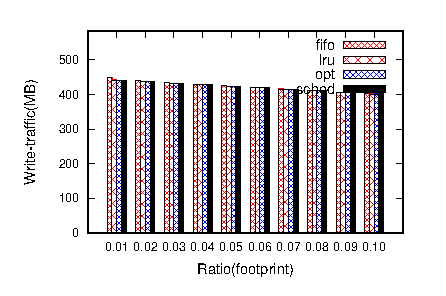
\includegraphics[width=0.24\textwidth]{./map-traffic/webserver_map.trc.eps}
	} 
    \subfloat[Linkbench]{
        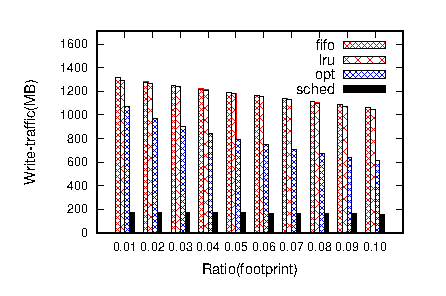
\includegraphics[width=0.24\textwidth]{./map-traffic/linkbench_r_map.trc.eps}
	}
	\subfloat[YCSB-00]{
        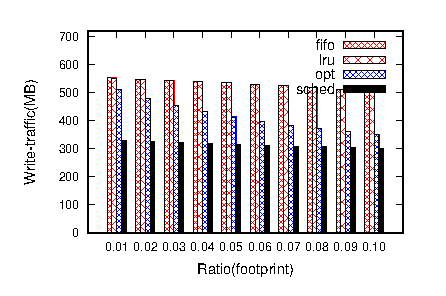
\includegraphics[width=0.24\textwidth]{./map-traffic/ssdtrace-00.blk_w.trc.eps}
	} \\
	\subfloat[YCSB-01]{
        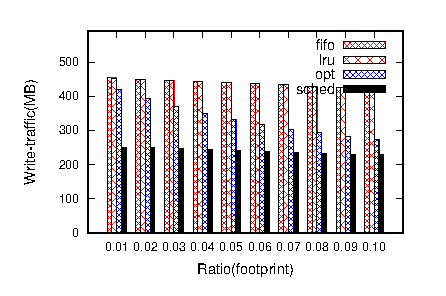
\includegraphics[width=0.24\textwidth]{./map-traffic/ssdtrace-01.blk_w.trc.eps}
	} 
	\subfloat[Systor-16LUN3]{
        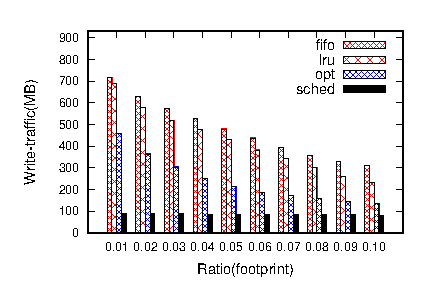
\includegraphics[width=0.24\textwidth]{./map-traffic/2016021616-LUN3.csv_w.trc.eps}
	} 
	\subfloat[Systor-16LUN4]{
        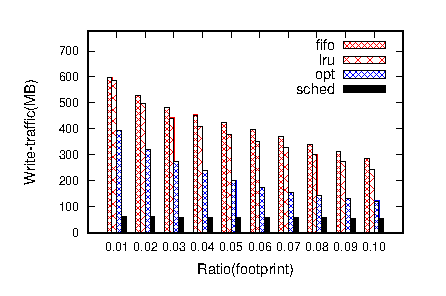
\includegraphics[width=0.24\textwidth]{./map-traffic/2016021616-LUN4.csv_w.trc.eps}
	} 
	\subfloat[Systor-18LUN3]{
        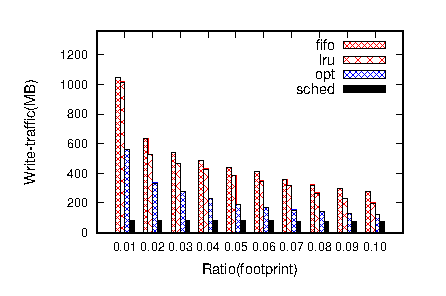
\includegraphics[width=0.24\textwidth]{./map-traffic/2016021618-LUN3.csv_w.trc.eps}
	} 

	\caption{\textbf{Write-back traffic of mapping table.}
%		\st{The \texttt{fillrandom} inserts items with random keys for each thread,
%    and the \texttt{overwrite} updates existing values in random order.
%    Both represent a put operation.
%    The \texttt{readrandom} retrieves items randomly,
%    and the \texttt{seekrandom} performs random seeks and queries the next ten items.}
	 }\label{fig_maptbl_write_traffic}
\end{figure*} 



%\begin{figure*}[!bt]
%    \centering{}
%    \subfloat[Fileserver]{
%        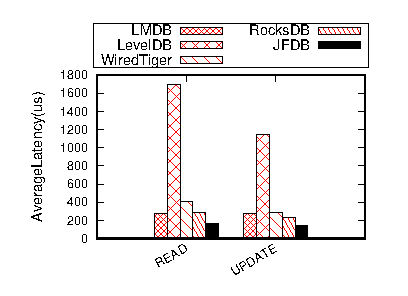
\includegraphics[width=0.24\textwidth]{./ycsb_graph/ycsb_16_a.eps}
%	}
%    \subfloat[Webserver]{
%        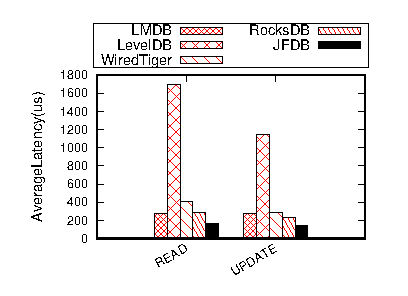
\includegraphics[width=0.24\textwidth]{./ycsb_graph/ycsb_16_a.eps}
%	} 
%    \subfloat[Linkbench]{
%        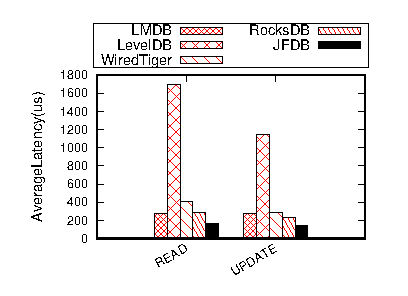
\includegraphics[width=0.24\textwidth]{./ycsb_graph/ycsb_16_a.eps}
%	}
%	\subfloat[YCSB-00]{
%        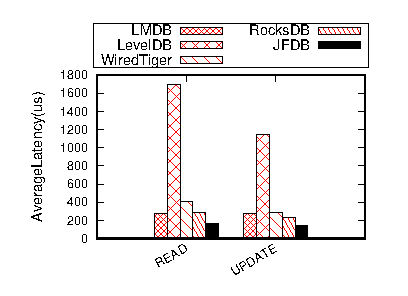
\includegraphics[width=0.24\textwidth]{./ycsb_graph/ycsb_16_a.eps}
%	} \\
%	\subfloat[YCSB-01]{
%        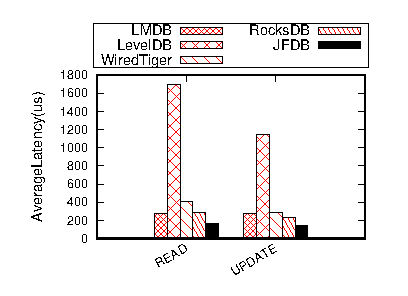
\includegraphics[width=0.24\textwidth]{./ycsb_graph/ycsb_16_a.eps}
%	} 
%	\subfloat[Systor-16LUN3]{
%        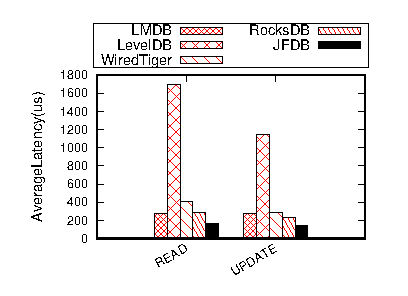
\includegraphics[width=0.24\textwidth]{./ycsb_graph/ycsb_16_a.eps}
%	} 
%	\subfloat[Systor-16LUN4]{
%        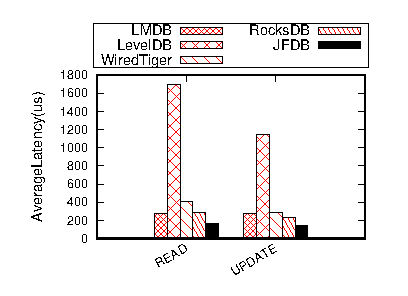
\includegraphics[width=0.24\textwidth]{./ycsb_graph/ycsb_16_a.eps}
%	} 
%	\subfloat[Systor-18LUN3]{
%        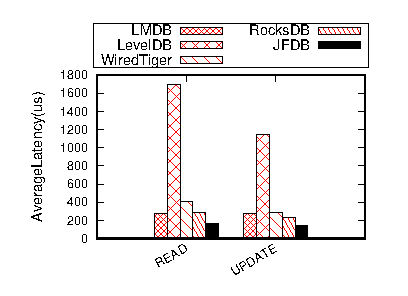
\includegraphics[width=0.24\textwidth]{./ycsb_graph/ycsb_16_a.eps}
%	} 
%
%	\caption{\textbf{Write-back traffic of mapping table.}
%		\st{The \texttt{fillrandom} inserts items with random keys for each thread,
%    and the \texttt{overwrite} updates existing values in random order.
%    Both represent a put operation.
%    The \texttt{readrandom} retrieves items randomly,
%    and the \texttt{seekrandom} performs random seeks and queries the next ten items.}
%	 }\label{fig_write_traffic}
%\end{figure*} 


